%%%%%%%%%%%%%%%%%%%%%%%%%%%%%%%%%%%%%%%%%%%%%%%%%%%%%%%%%%%%%%%%%%%%%%%%%%%%%%%
% APPENDIX H: REF-SEGMENTATION-HEURISTICS
% Quick Decision Guides and Rules of Thumb for Behavioral Segmentation
%%%%%%%%%%%%%%%%%%%%%%%%%%%%%%%%%%%%%%%%%%%%%%%%%%%%%%%%%%%%%%%%%%%%%%%%%%%%%%%
%
% CATEGORY: REF (Reference - Practical Aids & Decision Tools)
% Module: BCM2_10_SEG_HEUR (Segmentation Heuristics & Rules of Thumb)
% Version: 1.0 (January 2026)
% Status: Final
% Language: English/German (bilingual quick reference)
%
% PURPOSE:
% Provide practitioners with quick decision heuristics, diagnostic trees, and
% rules of thumb for segmentation work. Complements the formal theory in
% Appendix BA and the practical examples in Chapter 14 with fast, actionable
% guidance when designing, diagnosing, or refining segmentation studies.
%
%%%%%%%%%%%%%%%%%%%%%%%%%%%%%%%%%%%%%%%%%%%%%%%%%%%%%%%%%%%%%%%%%%%%%%%%%%%%%%%

\chapter{REF-SEGMENTATION-HEURISTICS: Quick Decision Guides}
\label{app:ref-seg-heuristics}

%------------------------------------------------------------------------------
% HEADER BLOCK
%------------------------------------------------------------------------------

\begin{tcolorbox}[colback=gray!5!white, colframe=gray!75!black,
    title=Appendix HHH: Header Block]

\noindent
\textbf{Code:} HHH \quad \textbf{Category:} REF-SEGMENTATION-HEURISTICS \\
\textbf{Module:} BCM2\_10\_SEG\_HEUR \quad \textbf{Version:} 1.0 (January 2026) \\
\textbf{Status:} Final \quad \textbf{Language:} English (German terms included)

\vspace{0.5em}

\noindent
\textbf{Description:}
Quick heuristics, decision trees, and rules of thumb for practicing segmentation. Provides practitioners with fast diagnostic guides when facing common decisions: How many clusters? Which clustering method? How to diagnose problems? When does segmentation add value? This appendix is designed for practical use during project work.

\end{tcolorbox}

%------------------------------------------------------------------------------
% CHAPTER LINKAGE BOX
%------------------------------------------------------------------------------

\begin{tcolorbox}[colback=purple!5!white, colframe=purple!75!black,
    title=Chapter Linkage]

\textbf{Primary Chapter:}
\begin{itemize}[nosep]
\item Chapter 14: Behavioral Change Segments (§2 Identification Methods, §3 Examples, §4 Diagnostics)
\end{itemize}

\textbf{Secondary Chapters:}
\begin{itemize}[nosep]
\item Chapter 15: Integration Framework (uses segmentation diagnostics)
\end{itemize}

\textbf{Reading Guide:}
\begin{itemize}[nosep]
\item For theory: Read Appendix BA (formal axioms) first
\item For practical examples: Chapter 14 shows step-by-step application
\item For quick decisions during a project: This appendix provides decision tables
\item For diagnostic troubleshooting: Go directly to relevant section below
\end{itemize}

\end{tcolorbox}

%------------------------------------------------------------------------------
% QUICK REFERENCE BOX
%------------------------------------------------------------------------------

\begin{tcolorbox}[colback=yellow!10!white, colframe=yellow!75!black,
    title=Quick Reference: The 4 Heuristics]

\begin{itemize}[nosep]
\item \textbf{H1: Cluster Count Selection} -- How to choose $k$
\item \textbf{H2: Heterogeneity Diagnosis} -- What does cluster size distribution reveal?
\item \textbf{H3: Leverage Matching} -- Is AvgLeverage sufficient? ($\geq 0.4$ = good)
\item \textbf{H4: Problem Diagnosis} -- When segmentation disappoints, where's the fault?
\end{itemize}

\textbf{Key Rule of Thumb:} AvgLeverage $\geq 0.4$ $\Rightarrow$ expect effects. AvgLeverage $< 0.3$ $\Rightarrow$ redesign interventions.

\end{tcolorbox}

\vspace{1em}

%==============================================================================
% ABSTRACT
%==============================================================================

\begin{tcolorbox}[colback=blue!5!white, colframe=blue!75!black,
    title=Abstract]

This appendix translates the formal theory of Appendix BA and the practical operationalization of Chapter 14 into \textbf{actionable decision heuristics}. It is designed for use \textit{during active project work}, when practitioners need rapid guidance on key decisions: How many clusters? Which method? Is leverage sufficient? What went wrong?

Organized as a collection of 6 heuristics covering the full segmentation workflow (planning → analysis → troubleshooting), this appendix provides decision trees, diagnostic tables, quick reference rules, and worked examples that can be applied immediately without deep theory study.

\end{tcolorbox}

\vspace{1em}

%==============================================================================
% FUNDAMENTAL QUESTION
%==============================================================================

\section{Fundamental Question}
\label{sec:h-fundamental}

\textbf{How can practitioners rapidly make six key segmentation decisions (cluster count, heterogeneity diagnosis, leverage matching, problem diagnosis, method selection, intervention design) without requiring deep statistical expertise or extensive time investment?}

This appendix answers this question by providing 6 decision heuristics---rules of thumb, diagnostic trees, and reference tables---that operationalize the formal framework of Appendix BA for real-world use.

\vspace{1em}

%==============================================================================
% THEORY
%==============================================================================

\section{Theory: Why These Heuristics?}
\label{sec:h-theory}

Appendix BA formalizes segment emergence from heterogeneity (Axioms 1-9) and establishes how theory externalization and diagnostic refinement improve segmentation practice (Axioms 10-13). However, formal theory requires time to apply and study. In practice, practitioners need \textbf{quick decision procedures} that distill the formal results into actionable rules.

\textbf{Key Insight from BA:} Three quantities determine segmentation success:

\begin{enumerate}
\item \textbf{Cluster count ($k$):} Should be data-driven and context-dependent, not fixed a priori
\item \textbf{Cluster homogeneity:} Measured by leverage profiles ($\ell_k^d$) and validated by intervention response
\item \textbf{Intervention matching:} Measured by AvgLeverage ($\geq 0.4$ predicts success; $< 0.3$ predicts failure)
\end{enumerate}

Each heuristic below targets one or more of these quantities, providing rules of thumb that practitioners can apply in minutes.

\vspace{1em}

%==============================================================================
% RESULTS
%==============================================================================

\section{Results: Six Operational Heuristics}
\label{sec:h-results}

\textbf{H1 (Cluster Count Selection):} Use domain knowledge (Rogers, adoption type) combined with silhouette score validation. If silhouette $> 0.6$ and clusters align with domain theory, $k$ is likely optimal.

\textbf{H2 (Heterogeneity Diagnosis):} Compute coefficient of variation (CV) of cluster sizes. CV $< 0.4$ (normal), CV $0.4$-$1.2$ (skewed), CV $> 1.2$ (polarized). CV predicts both clustering method performance and intervention design complexity.

\textbf{H3 (Leverage Matching):} Calculate AvgLeverage from leverage profiles. If AvgLeverage $\geq 0.4$, expect Cohen's $d \approx 0.12$-$0.18$. If AvgLeverage $< 0.3$, redesign interventions before launching.

\textbf{H4 (Problem Diagnosis):} When results disappoint, compare observed AvgLeverage to predicted. Diagnosis follows three cases: (a) observed $\ll$ predicted = intervention matching failure; (b) observed $\approx$ predicted = correct leverage but barriers remain; (c) both high but no effect = implementation fidelity problem.

\textbf{H5 (Method Selection):} Choose clustering algorithm based on heterogeneity type: normal (k-means), skewed (hierarchical), polarized (Gaussian Mixture Models), unknown (BIC validation).

\textbf{H6 (Intervention Design):} Map leverage profiles to intervention design intensities: $\ell^d > 0.6 \Rightarrow \delta_I^d = 0.8$-$1.0$; $\ell^d 0.3$-$0.6 \Rightarrow \delta_I^d = 0.4$-$0.6$; $\ell^d < 0.3 \Rightarrow \delta_I^d = 0$.

\vspace{1em}

%==============================================================================
% HEURISTIC 1: CLUSTER COUNT SELECTION
%==============================================================================

\section{Heuristic 1: Cluster Count Selection --- How Many Segments?}
\label{sec:h1-cluster-count}

\textbf{The Question:} Given data, how many clusters $k$ should I extract?

\textbf{The Problem:} Using wrong $k$ wastes resources (too many tiny clusters) or misses important structure (too few large clusters). The Elbow Method alone is ambiguous. Practitioners need quick guidance.

\subsection{The Decision Tree}

\begin{center}
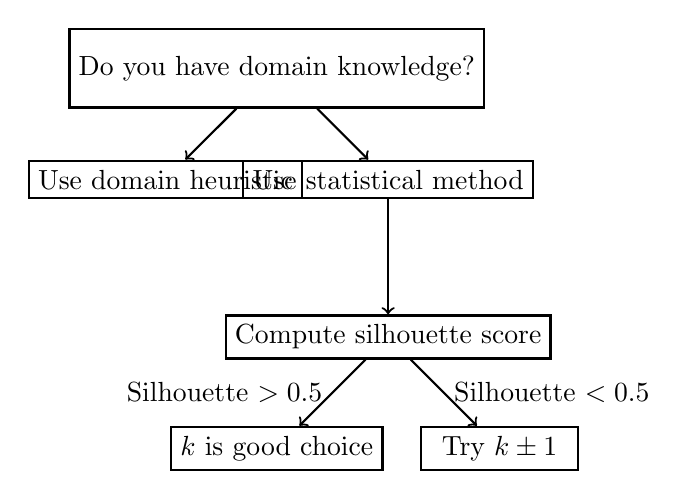
\begin{tikzpicture}[node distance=2cm, auto, thick]
% Start
\node (start) [rectangle, draw, minimum width=3cm, minimum height=1cm] {Do you have domain knowledge?};
\node (dk_yes) [rectangle, draw, below left of=start, minimum width=2.5cm] {Use domain heuristic};
\node (dk_no) [rectangle, draw, below right of=start, minimum width=2.5cm] {Use statistical method};

\node (silhouette) [rectangle, draw, below of=dk_no, minimum width=3cm] {Compute silhouette score};
\node (sil_high) [rectangle, draw, below left of=silhouette, minimum width=2cm] {$k$ is good choice};
\node (sil_low) [rectangle, draw, below right of=silhouette, minimum width=2cm] {Try $k \pm 1$};

\draw [->] (start) -- (dk_yes);
\draw [->] (start) -- (dk_no);
\draw [->] (dk_no) -- (silhouette);
\draw [->] (silhouette) -- node[left] {Silhouette $> 0.5$} (sil_high);
\draw [->] (silhouette) -- node[right] {Silhouette $< 0.5$} (sil_low);
\end{tikzpicture}
\end{center}

\subsection{Quick Reference Table}

\begin{table}[h]
\centering
\small
\begin{tabular}{llll}
\toprule
\textbf{Domain Knowledge?} & \textbf{Silhouette Score} & \textbf{Recommendation} & \textbf{Action} \\
\midrule
Yes & --- & Use domain knowledge $k$ & Proceed with confidence \\
Yes & $> 0.5$ & Confirm with data & Domain + data agree ✓ \\
Yes & $< 0.5$ & Reconsider domain $k$ & Data suggests different structure \\
No & $> 0.6$ & Use indicated $k$ & High confidence \\
No & $0.4$-$0.6$ & Use indicated $k$ & Moderate confidence \\
No & $< 0.4$ & Try $k \pm 1$ & Explore alternatives \\
\bottomrule
\end{tabular}
\caption{Quick decision table for choosing $k$}
\label{tab:h1-cluster-count}
\end{table}

\subsection{Domain Heuristics (Use These If Available)}

\begin{itemize}[nosep]
\item \textbf{Environmental behavior (adoption):} Start with $k = 5$ (Rogers)
\item \textbf{Health behavior (mandatory):} Start with $k = 2$-$3$ (Compliers/Skeptics/Defiant)
\item \textbf{Financial behavior:} Start with $k = 3$-$4$ (Risk-seekers/Pragmatists/Risk-averse)
\item \textbf{Technology usage (established):} Start with $k = 2$-$3$ (Heavy/Moderate/Light users)
\end{itemize}

%==============================================================================
% HEURISTIC 2: HETEROGENEITY DIAGNOSIS
%==============================================================================

\section{Heuristic 2: Heterogeneity Diagnosis --- What's the Population's Structure?}
\label{sec:h2-heterogeneity}

\textbf{The Question:} Your cluster sizes are $\{70\%, 20\%, 10\%\}$. Normal? Problematic? What does this tell you?

\textbf{Key Metric:} Coefficient of Variation: $CV = \sigma_{|C_k|} / \bar{|C_k|}$ where $\bar{|C_k|} = N/k$

\subsection{The Diagnostic Grid}

\begin{table}[h]
\centering
\small
\begin{tabular}{ccccll}
\toprule
\textbf{CV} & \textbf{Max/Min Ratio} & \textbf{Pattern Type} & \textbf{Distribution} & \textbf{Interpretation} & \textbf{Action} \\
\midrule
$0.2$-$0.4$ & $< 10$ & Balanced & Normal & Natural structure & Use standard k-means \\
$0.4$-$0.7$ & $10$-$50$ & Slightly skewed & Near-normal & Mild polarization & Hierarchical clustering \\
$0.7$-$1.2$ & $50$-$200$ & Moderately skewed & Skewed right & Some segments small & Use BIC to validate \\
$> 1.2$ & $> 200$ & Highly polarized & Bimodal & Major vs. minor & Gaussian Mixture Models \\
\bottomrule
\end{tabular}
\caption{Heterogeneity diagnosis grid}
\label{tab:h2-heterogeneity}
\end{table}

\subsection{What to Do in Each Case}

\textbf{Normal Distribution ($CV < 0.4$):}
- Segmentation will be clean and stable
- Standard k-means or hierarchical clustering works well
- Segment-specific interventions likely to be effective
- Confidence: HIGH

\textbf{Skewed Distribution ($0.4 < CV < 1.0$):}
- One cluster is dominant; others are minority
- Interventions for minorities may need special care
- Don't force equal resources across clusters
- Confidence: MODERATE

\textbf{Polarized Distribution ($CV > 1.0$):}
- Population has two distinct camps
- ``Middle ground'' messaging will fail
- Design separate interventions for major/minor camps
- Can't bridge the gap; can only address each independently
- Confidence: LOW -- be cautious about effect sizes

%==============================================================================
% HEURISTIC 3: LEVERAGE MATCHING
%==============================================================================

\section{Heuristic 3: Leverage Matching --- Is Your Intervention Matched?}
\label{sec:h3-leverage-matching}

\textbf{The Question:} I computed AvgLeverage = 0.35. Will my segmented intervention beat the control?

\textbf{Quick Rule of Thumb:}

\begin{center}
\begin{tcolorbox}[colback=blue!10!white, colframe=blue!75!black]

$$\text{Expected Effect} \approx \text{AvgLeverage} \times 0.3$$

If AvgLeverage = 0.35 $\Rightarrow$ expected effect $\approx 0.35 \times 0.3 = 0.10$ (small)

If AvgLeverage = 0.60 $\Rightarrow$ expected effect $\approx 0.60 \times 0.3 = 0.18$ (medium)

If AvgLeverage = 0.80 $\Rightarrow$ expected effect $\approx 0.80 \times 0.3 = 0.24$ (medium-large)

\end{tcolorbox}
\end{center}

\subsection{Decision Table}

\begin{table}[h]
\centering
\small
\begin{tabular}{lllll}
\toprule
\textbf{AvgLeverage} & \textbf{Interpretation} & \textbf{Expected d} & \textbf{Decision} & \textbf{Confidence} \\
\midrule
$< 0.3$ & Poor match & $< 0.09$ & Redesign first & LOW \\
$0.3$-$0.4$ & Weak match & $0.09$-$0.12$ & Borderline & LOW-MOD \\
$0.4$-$0.6$ & Moderate match & $0.12$-$0.18$ & Go ahead & MODERATE \\
$0.6$-$0.8$ & Strong match & $0.18$-$0.24$ & Go ahead & MODERATE-HIGH \\
$> 0.8$ & Very strong & $> 0.24$ & Go ahead & HIGH \\
\bottomrule
\end{tabular}
\caption{Leverage matching quick reference}
\label{tab:h3-leverage}
\end{table}

\textbf{Critical Decision Rule:} If AvgLeverage $< 0.4$, redesign your interventions before running the study. Low leverage won't overcome other friction.

%==============================================================================
% HEURISTIC 4: PROBLEM DIAGNOSIS
%==============================================================================

\section{Heuristic 4: Problem Diagnosis --- Why Didn't Segmentation Work?}
\label{sec:h4-diagnosis}

\textbf{The Question:} I pre-registered expecting effect size $d = 0.18$. I got $d = 0.02$. What went wrong?

\textbf{Diagnostic Decision Tree:}

\subsection{Step 1: Check AvgLeverage}

Compute actual leverage from study data. Compare to predicted leverage.

\begin{table}[h]
\centering
\small
\begin{tabular}{lll}
\toprule
\textbf{Observed AvgLeverage} & \textbf{Predicted was} & \textbf{Problem Type} \\
\midrule
$< 0.3$ & $> 0.5$ & Intervention matching failure \\
$0.3$-$0.6$ & $0.3$-$0.6$ & Segmentation quality OK, low effect unexpected \\
$> 0.6$ & $> 0.6$ & Both matched well, but no effect $\Rightarrow$ implementation/fidelity \\
\bottomrule
\end{tabular}
\caption{Diagnostic triage}
\label{tab:h4-diagnosis}
\end{table}

\subsection{Step 2: Root Cause Analysis}

\textbf{IF AvgLeverage observed $< 0.3$ and predicted $> 0.5$:}

\textbf{ROOT CAUSE:} Interventions didn't reach/resonate with clusters

\begin{itemize}[nosep]
\item \textbf{Symptom:} Intervention deployment failed (e.g., email campaign bounced, website content not seen)
\item \textbf{Fix:} Increase salience. Push interventions instead of pull. Use direct communication.
\item \textbf{Confidence:} HIGH -- almost certainly a delivery problem
\end{itemize}

\textbf{IF AvgLeverage observed $0.4$-$0.6$ and predicted $0.4$-$0.6$ but effect is still tiny:}

\textbf{ROOT CAUSE:} Intervention matching is correct, but something else is blocking

\begin{itemize}[nosep]
\item \textbf{Symptom:} Leverage is moderate; effect is still too small
\item \textbf{Check:} Implementation fidelity (did clusters actually receive what was promised?)
\item \textbf{Check:} Barriers beyond those in your leverage profile (cost, social disapproval, etc.)
\item \textbf{Fix:} Address barriers directly. Remove friction.
\item \textbf{Confidence:} MODERATE -- multiple possible causes
\end{itemize}

\textbf{IF AvgLeverage observed $> 0.6$ and predicted $> 0.6$ but effect is still near zero:}

\textbf{ROOT CAUSE:} Segmentation hypothesis may be wrong OR implementation was very poor

\begin{itemize}[nosep]
\item \textbf{Symptom:} Leverage is high but nothing happened
\item \textbf{Check:} Cluster quality. Run silhouette score. Are clusters actually homogeneous?
\item \textbf{Check:} Did treated group actually receive treatment? Check fidelity logs.
\item \textbf{Fix:} Either revalidate clusters OR rerun with better implementation
\item \textbf{Confidence:} LOW -- troubleshooting required
\end{itemize}

%==============================================================================
% DECISION FLOWCHART: THE COMPLETE DIAGNOSTIC
%==============================================================================

\section{Complete Diagnostic Flowchart}
\label{sec:h4-flowchart}

When results disappoint, use this flowchart:

\vspace{1em}

\begin{enumerate}
\item \textbf{Compute $\text{AvgLeverage}_{\text{observed}}$ from your data}
\item \textbf{Compare to $\text{AvgLeverage}_{\text{predicted}}$ from pre-registration}
\item \textbf{Use table below to diagnose}
\end{enumerate}

\begin{table}[h]
\centering
\small
\begin{tabular}{|l|l|l|l|}
\hline
\textbf{Predicted} & \textbf{Observed} & \textbf{Effect} & \textbf{DIAGNOSIS \& FIX} \\
\hline
High (0.6+) & Low (0.2-) & Null & Intervention matching failed. FIX: Increase salience, push instead of pull \\
\hline
Moderate (0.4) & Moderate (0.4) & Null/Small & Correct leverage, but barriers remain. FIX: Address specific barriers \\
\hline
Moderate (0.4) & Low (0.2) & Null & Intervention didn't reach clusters. FIX: Delivery problem. Retry with direct outreach \\
\hline
Low (0.2) & Low (0.2) & Null & Low leverage as expected. FIX: Choose higher-leverage dimensions or better interventions \\
\hline
High (0.6+) & High (0.6+) & Null & Segmentation itself may be wrong. FIX: Revalidate cluster quality or check implementation fidelity \\
\hline
\end{tabular}
\caption{Complete diagnostic table}
\label{tab:h4-complete}
\end{table}

%==============================================================================
% CLUSTERING METHOD SELECTION
%==============================================================================

\section{Heuristic 5: Clustering Method Selection --- Which Algorithm?}
\label{sec:h5-clustering-methods}

\textbf{The Question:} K-means vs. hierarchical vs. Gaussian Mixture? Which to use?

\begin{table}[h]
\centering
\small
\begin{tabular}{lllll}
\toprule
\textbf{Method} & \textbf{When to Use} & \textbf{Heterogeneity Type} & \textbf{Pros} & \textbf{Cons} \\
\midrule
\textbf{K-means} & Default choice & Normal/balanced & Fast, stable & Assumes spherical clusters \\
\textbf{Hierarchical} & Mixed sizes & Skewed dist. & Flexible, dendrograms & Slower, sensitive to linkage \\
\textbf{Gaussian Mix} & Polarized & Bimodal & Probabilistic, soft assign. & Complex, slow, needs tuning \\
\textbf{Spectral} & Non-convex & Any & Handles complex shapes & Slow for large $N$ \\
\bottomrule
\end{tabular}
\caption{Clustering method selection guide}
\label{tab:h5-methods}
\end{table}

\textbf{Quick Decision Rule:}

\begin{itemize}[nosep]
\item \textbf{$CV < 0.5$ (normal heterogeneity):} Use K-means. Fast and reliable.
\item \textbf{$0.5 < CV < 1.0$ (skewed):} Use hierarchical with Ward linkage.
\item \textbf{$CV > 1.0$ (polarized):} Use Gaussian Mixture Models to capture soft probabilities.
\item \textbf{Always validate:} Compute silhouette score. If $< 0.4$, try alternative method.
\end{itemize}

%==============================================================================
% INTERVENTION DESIGN HEURISTICS
%==============================================================================

\section{Heuristic 6: Intervention Design --- How to Target Leverage?}
\label{sec:h6-intervention-design}

\textbf{The Question:} My cluster has $\ell^S = 0.7$ (high Social), $\ell^F = 0.1$ (low Financial). How do I design?

\textbf{Quick Design Rule:}

\begin{table}[h]
\centering
\small
\begin{tabular}{lll}
\toprule
\textbf{Leverage ($\ell^d$)} & \textbf{Dimension Focus} & \textbf{Intervention Design Intensity ($\delta_I^d$)} \\
\midrule
$> 0.6$ & Must address & $\delta_I^d = 0.8$-$1.0$ (HIGH focus) \\
$0.3$-$0.6$ & Should address & $\delta_I^d = 0.4$-$0.6$ (MODERATE) \\
$< 0.3$ & Can ignore & $\delta_I^d = 0$-$0.2$ (LOW/skip) \\
\bottomrule
\end{tabular}
\caption{Leverage-to-design mapping}
\label{tab:h6-design}
\end{table}

\textbf{Example:} Your cluster has $\ell^S = 0.7, \ell^F = 0.1$

$\Rightarrow$ Design intervention with $\delta_I^S = 0.9$ (peer pressure, social proof), $\delta_I^F = 0.0$ (skip ROI messaging)

\textbf{Expected matching:} Leverage$(I, C_k) = 0.7 \times 0.9 + 0.1 \times 0.0 = 0.63$ ✓

%==============================================================================
% SUMMARY
%==============================================================================

\section{Summary: When to Use Each Heuristic}
\label{sec:h-summary}

\begin{tcolorbox}[colback=green!10!white, colframe=green!75!black,
    title=Summary: Quick Decision Guide]

\textbf{During Project Planning:}
\begin{enumerate}[nosep]
\item \textbf{H1:} How many clusters should I extract?
\item \textbf{H5:} Which clustering method should I use?
\end{enumerate}

\textbf{During Analysis:}
\begin{enumerate}[nosep]
\item \textbf{H2:} What does my cluster size distribution reveal?
\item \textbf{H6:} How should I design interventions for each cluster's leverage?
\item \textbf{H3:} Is my AvgLeverage sufficient? Can I expect effects?
\end{enumerate}

\textbf{During Troubleshooting (When Results Disappoint):}
\begin{enumerate}[nosep]
\item \textbf{H4:} What went wrong? Use diagnostic flowchart to identify root cause.
\end{enumerate}

\end{tcolorbox}

%==============================================================================
% GLOSSARY SECTION
%==============================================================================

\section{Glossary: Key Terms in This Appendix}
\label{sec:h-glossary}

See \textbf{Appendix G: Glossary of Terms} for comprehensive notation and concepts. Key terms used in this appendix:

\begin{itemize}[nosep]
\item \textbf{$k$ (cluster count):} Number of behavioral segments to extract
\item \textbf{$\ell_k^d$ (leverage in dimension $d$):} Variance of utility dimension $d$ within cluster $k$, normalized
\item \textbf{$\text{AvgLeverage}$:} Average leverage across all clusters and matched dimensions
\item \textbf{$\delta_I^d$ (intervention design intensity):} Degree to which intervention $I$ targets dimension $d$
\item \textbf{CV (coefficient of variation):} Standard deviation of cluster sizes divided by mean cluster size
\item \textbf{Silhouette score:} Cluster quality metric (range: -1 to 1; > 0.6 indicates good separation)
\item \textbf{Heterogeneity distribution:} Distribution of preferences across population (normal, skewed, bimodal, polarized)
\end{itemize}

%==============================================================================
% CRITICAL FOUNDATIONS
%==============================================================================

\section{Critical Foundations}
\label{sec:h-foundations}

These heuristics rest on five critical foundations from Appendix BA:

\begin{enumerate}
\item \textbf{Axiom 1 (Heterogeneity is universal):} Any population of sufficient size ($N > 100$) contains meaningful preference heterogeneity (Appendix BA, §2.1)

\item \textbf{Axiom 4 (Behavioral homogeneity within clusters):} Valid clusters exhibit within-cluster behavioral homogeneity and can be identified by different intervention responses (Appendix BA, §2.4)

\item \textbf{Axiom 8-9 (Leverage matching):} Segment-specific interventions achieve higher expected effects when targeting each segment's leverage profile (Appendix BA, §3)

\item \textbf{Axiom 12 (Diagnostic refinement):} Diagnostic procedures using AvgLeverage as the key discriminator enable practitioners to distinguish intervention-matching failures from segmentation failures (Appendix BA, §4.3)

\item \textbf{Axiom 13 (Cumulative science):} Systematic documentation of segmentation decisions and refined diagnoses builds cumulative knowledge across projects (Appendix BA, §4.4)
\end{enumerate}

%==============================================================================
% OPEN ISSUES & FUTURE RESEARCH
%==============================================================================

\section{Open Issues}
\label{sec:h-open-issues}

While these heuristics provide actionable guidance, several research questions remain open:

\begin{enumerate}
\item \textbf{Dynamic cluster membership:} How stable are segment memberships over time? Should practitioners re-segment regularly or use dynamic clustering models?

\item \textbf{Multi-dimensional leverage:} When multiple utility dimensions have high leverage (e.g., $\ell_k^S = 0.6$ and $\ell_k^F = 0.55$), should interventions address both or prioritize? Optimization rules unclear.

\item \textbf{Intervention interaction effects:} Does combining cluster-specific interventions produce additive or multiplicative effects? May vary by context.

\item \textbf{Optimal leverage threshold:} Is AvgLeverage $\geq 0.4$ universally optimal? May depend on outcome variability and implementation context.

\item \textbf{CV-method-performance relationship:} Does the relationship between CV and clustering method performance (H5) hold across all domains? Empirical validation needed.
\end{enumerate}

For ongoing research, practitioners should document results systematically in the FFF (Framework Falsification \& Feedback) registry (see Appendix G).

\vspace{1em}

%==============================================================================
% REFERENCES
%==============================================================================

\section{References}
\label{sec:h-references}

This appendix provides practical distillations of concepts formalized in:

\begin{itemize}[nosep]
\item \textbf{Axioms 1-9:} Appendix BA (Formal Segmentation Genesis)
\item \textbf{Clustering Methods:} Chapter 14, Section Practical Identification Methods
\item \textbf{Leverage Matching:} Appendix BA, Axioms 8-9
\item \textbf{Diagnostic Framework:} Appendix BA, Axiom 12; Chapter 14, Section Axioms 10-13
\end{itemize}

For theoretical justification of any heuristic, consult the primary sources above.

\vspace{1em}

\noindent
\cite{rogers2003diffusion, angrist2010mostly, thaler2008nudge}

\vspace{0.5em}

\noindent
\nocite{bcm_master}

%==============================================================================
% CROSS-REFERENCE FOOTER
%==============================================================================

\begin{tcolorbox}[colback=white, colframe=black, title=Cross-Reference Footer]

\textbf{This appendix connects to:}
\begin{itemize}[nosep]
\item Chapter 14: All sections (provides practical operationalization)
\item Appendix BA: All axioms (theoretical grounding)
\item Appendix G: Glossary (notation and terminology)
\end{itemize}

\textbf{Use this appendix:}
\begin{itemize}[nosep]
\item As quick reference during segmentation project work
\item For troubleshooting when results disappoint
\item To train new team members on standard procedures
\end{itemize}

\end{tcolorbox}

\end{document}
